\documentclass[french,a4paper]{article}
\setcounter{tocdepth}{4}
\setcounter{secnumdepth}{4}
\usepackage{float}
\usepackage{graphicx}
\usepackage{hyperref}
\usepackage{pdfpages}
\renewcommand{\contentsname}{Table des matières}
\newcommand{\tabitem}{\textbullet~~}
\newcommand{\HRule}{\rule{\linewidth}{0.5mm}}
\usepackage{multirow}
\graphicspath{{img/}}
\title{PPII}
\usepackage[bottom=2.5cm,top=2.5cm,left=2.5cm,right=2.5cm]{geometry}
\usepackage{textcomp}
\usepackage{amsmath}
\setcounter{MaxMatrixCols}{20}
\author{Noé Steiner - Alexis Marcel - Lucas Laurent - Mathias Aurand-Augier}
\date{Mai 2023}
\begin{document}

%\maketitle

\begin{titlepage}
    \begin{center}

        
\includegraphics[width=0.5\textwidth]{tele_univ.png}

        \textsc{\Large Rapport final de Projet Pluridisciplinaire d'Informatique Intégrative 2}\\[1.5cm]

        \HRule \\[0.4cm]
        { \huge \bfseries Optimisation trajet voitures électriques\\[0.4cm] }

        \HRule \\[2cm]

        \begin{minipage}{0.4\textwidth}
            \begin{flushleft} \large
                Alexis MARCEL\\
                Lucas LAURENT\\
                Noé STEINER\\
                Mathias AURAND-AUGIER\\
            \end{flushleft}
        \end{minipage}
        \begin{minipage}{0.4\textwidth}
            \begin{flushright} \large
                \emph{Responsable du module :}\\
                Olivier FESTOR\\
                Anne-Claire HEURTEL\\
                Gerald OSTER\\
            \end{flushright}
        \end{minipage}

        \vfill

        {\large 23 Mai 2023}

    \end{center}
\end{titlepage}
\newpage
\tableofcontents
\newpage
\section{Contexte du projet}
Ce rapport rend compte du Projet Pluridisciplinaire d’Informatique Intégrative dans le cadre de la première année du cycle ingénieur à TELECOM Nancy.
L’objectif de ce projet est de concevoir, en groupe, un algorithme permettant de trouver les itinéraires les plus optimaux pour les conducteurs de voitures électriques.
\section{Introduction}
Dans un contexte où la mobilité durable et la réduction des émissions de gaz à effet 
de serre sont devenues des enjeux majeurs, cette solution se présente comme une réponse prometteuse. En utilisant des algorithmes avancés et des 
données en temps réel, ce projet cherche à trouver les itinéraires les plus optimaux en termes de distance, de temps et de disponibilité des 
bornes de recharge pour les conducteurs de voitures électriques. 
\section{Conception}
\subsection{Cahier des charges}
On cherche à fabriquer un algorithme qui répond aux éxigences suivantes :
\subsection{Choix de la structure de données adapté}
Pour parvenir à choisir la structure de données optimale pour notre projet d'optimisation de trajet pour voitures électriques, nous avons exploré 
différentes options. Notre objectif était de trouver une structure de données qui puisse représenter 
efficacement les connexions entre les différentes stations, tout en facilitant les calculs d'itinéraires optimaux.

Nous avons commencé par étudier les structures de données vues en cours tels que les listes, les arbres et les graphes. Nous avons d'abord envisagé 
les arbres. Cependant, nous avons réalisé que cette structures ne convenait pas à notre cas d'utilisation, car elles 
ne permettaient pas de représenter efficacement toutes les connexions entre toutes les stations. Nous avons donc choisi de réprésenter notre problème
avec un graphe.

Dans notre approche, chaque nœud du graphe représente ainsi une station spécifique, ou une borne de recharge et les arêtes du graphe représentent 
les connexions entre ces positions, et donc les routes même si nous avons supposé que nous travaillions en vol d'oiseau pour simplifier le probleme.

L'utilisation des graphes nous permet de bénéficier d'algorithmes de recherche de chemin bien établis, tels que l'algorithme de Dijkstra que nous avons
étudié en cours de MSED ou l'algorithme A*, plus efficace mais aussi plus difficile à mettre en oeuvre. 

\subsection{choix de l'algorithmes de recherche de chemin optimal}
Au vue des contraintes qui s'imposait pour le projet notamment la contrainte de temps, nous avons choisi d'utiliser l'algorithme de Dijkstra 
pour notre projet, puisqu'il s'agit de l'algorithme que nous avions étudié en cours. 

\section{Gestion de projet}
\subsection{Équipe de projet}
Ce projet est un projet local réalisé en groupe de 4 personnes~:
\begin{itemize} 
    \item Alexis MARCEL
    \item Lucas LAURENT
    \item Noé STEINER
    \item Mathias AURAND-AUGIER
\end{itemize}
Le comité de pilotage est constitué de~:
\begin{itemize}
    \item Anne-Claire HEURTEL
    \item Olivier FESTOR
    \item Gérald OSTER
\end{itemize}
Ces personnes constituent les parties prenantes de notre projet ainsi que les acteurs influents sur le livrables.
\begin{figure}[H]
    \centering
    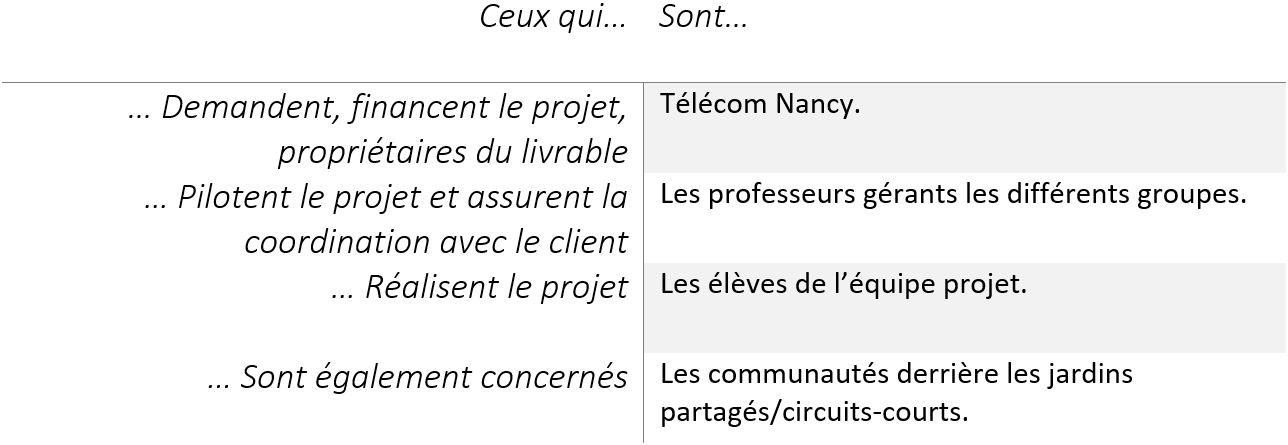
\includegraphics[width=0.75\textwidth]{img/parties_prenantes.png}
    \caption{Parties prenantes}
\end{figure}
\subsection{Organisation au sein de l’équipe projet}
Nous avons réalisé plusieurs réunions, en présentiel dans les locaux de Télécom Nancy mais la plupart de notre collaboration a eu lieu sur Discord. Ces réunions nous ont permis de mettre en commun nos avancées régulièrement, de partager nos connaissances sur des problématiques et de nous organiser de manière optimale.
En plus des réunions d'avancement règulières, nous avons également réalisé des réunions techniques afin de résoudre un problème ou bien de réflechir à la conception.
Les comptes rendus des réunions réalisées sont présents dans l’\hyperlink{annexe1}{Annexe 1}.

Contrairement au premier projet, nous avons choisi de travailler cette fois ci tous ensemble plutot que individuellement. Nous avons donc utiliser une 
application pour que nous puissons tous modifier le code en même temps, ce qui nous a permis de tous travailler sur le même code en même temps.

Ensuite, nous avons utilisé GitLab pour gérer les différentes versions du développement de notre application, ainsi que les différentes 
branches nous permettant de travailler simultanément sans conflit.

Enfin, la rédaction des differents comptes rendu de réunion et des rapports ont été rédigé en \LaTeX.

\subsection{Objectifs SMART}
La méthode SMART que l'on rappelle ci-dessous nous a permis de définir nos différents objectifs :

\begin{figure}[H]
    \centering
    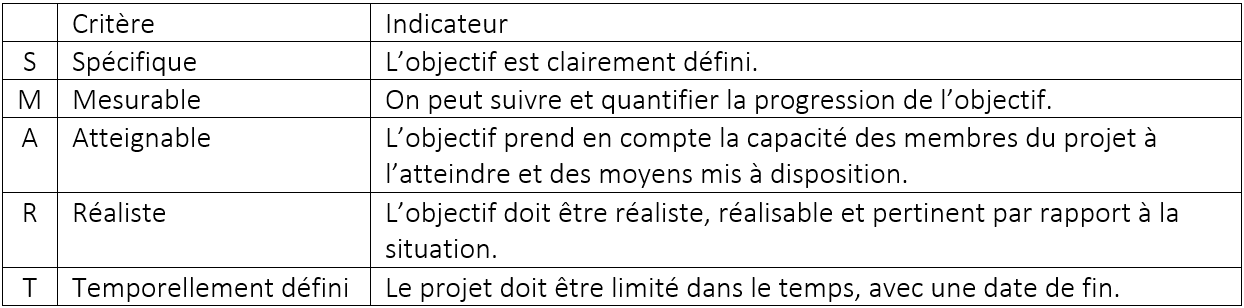
\includegraphics[width=1\textwidth]{img/SMART.png}
    \caption{Objectifs SMART}
\end{figure}

\subsection{Matrice des objectifs}
Nous avons conçu, à l'aide de la méthode SMART, la matrice des objectifs suivante :

\begin{figure}[H]
    \centering
    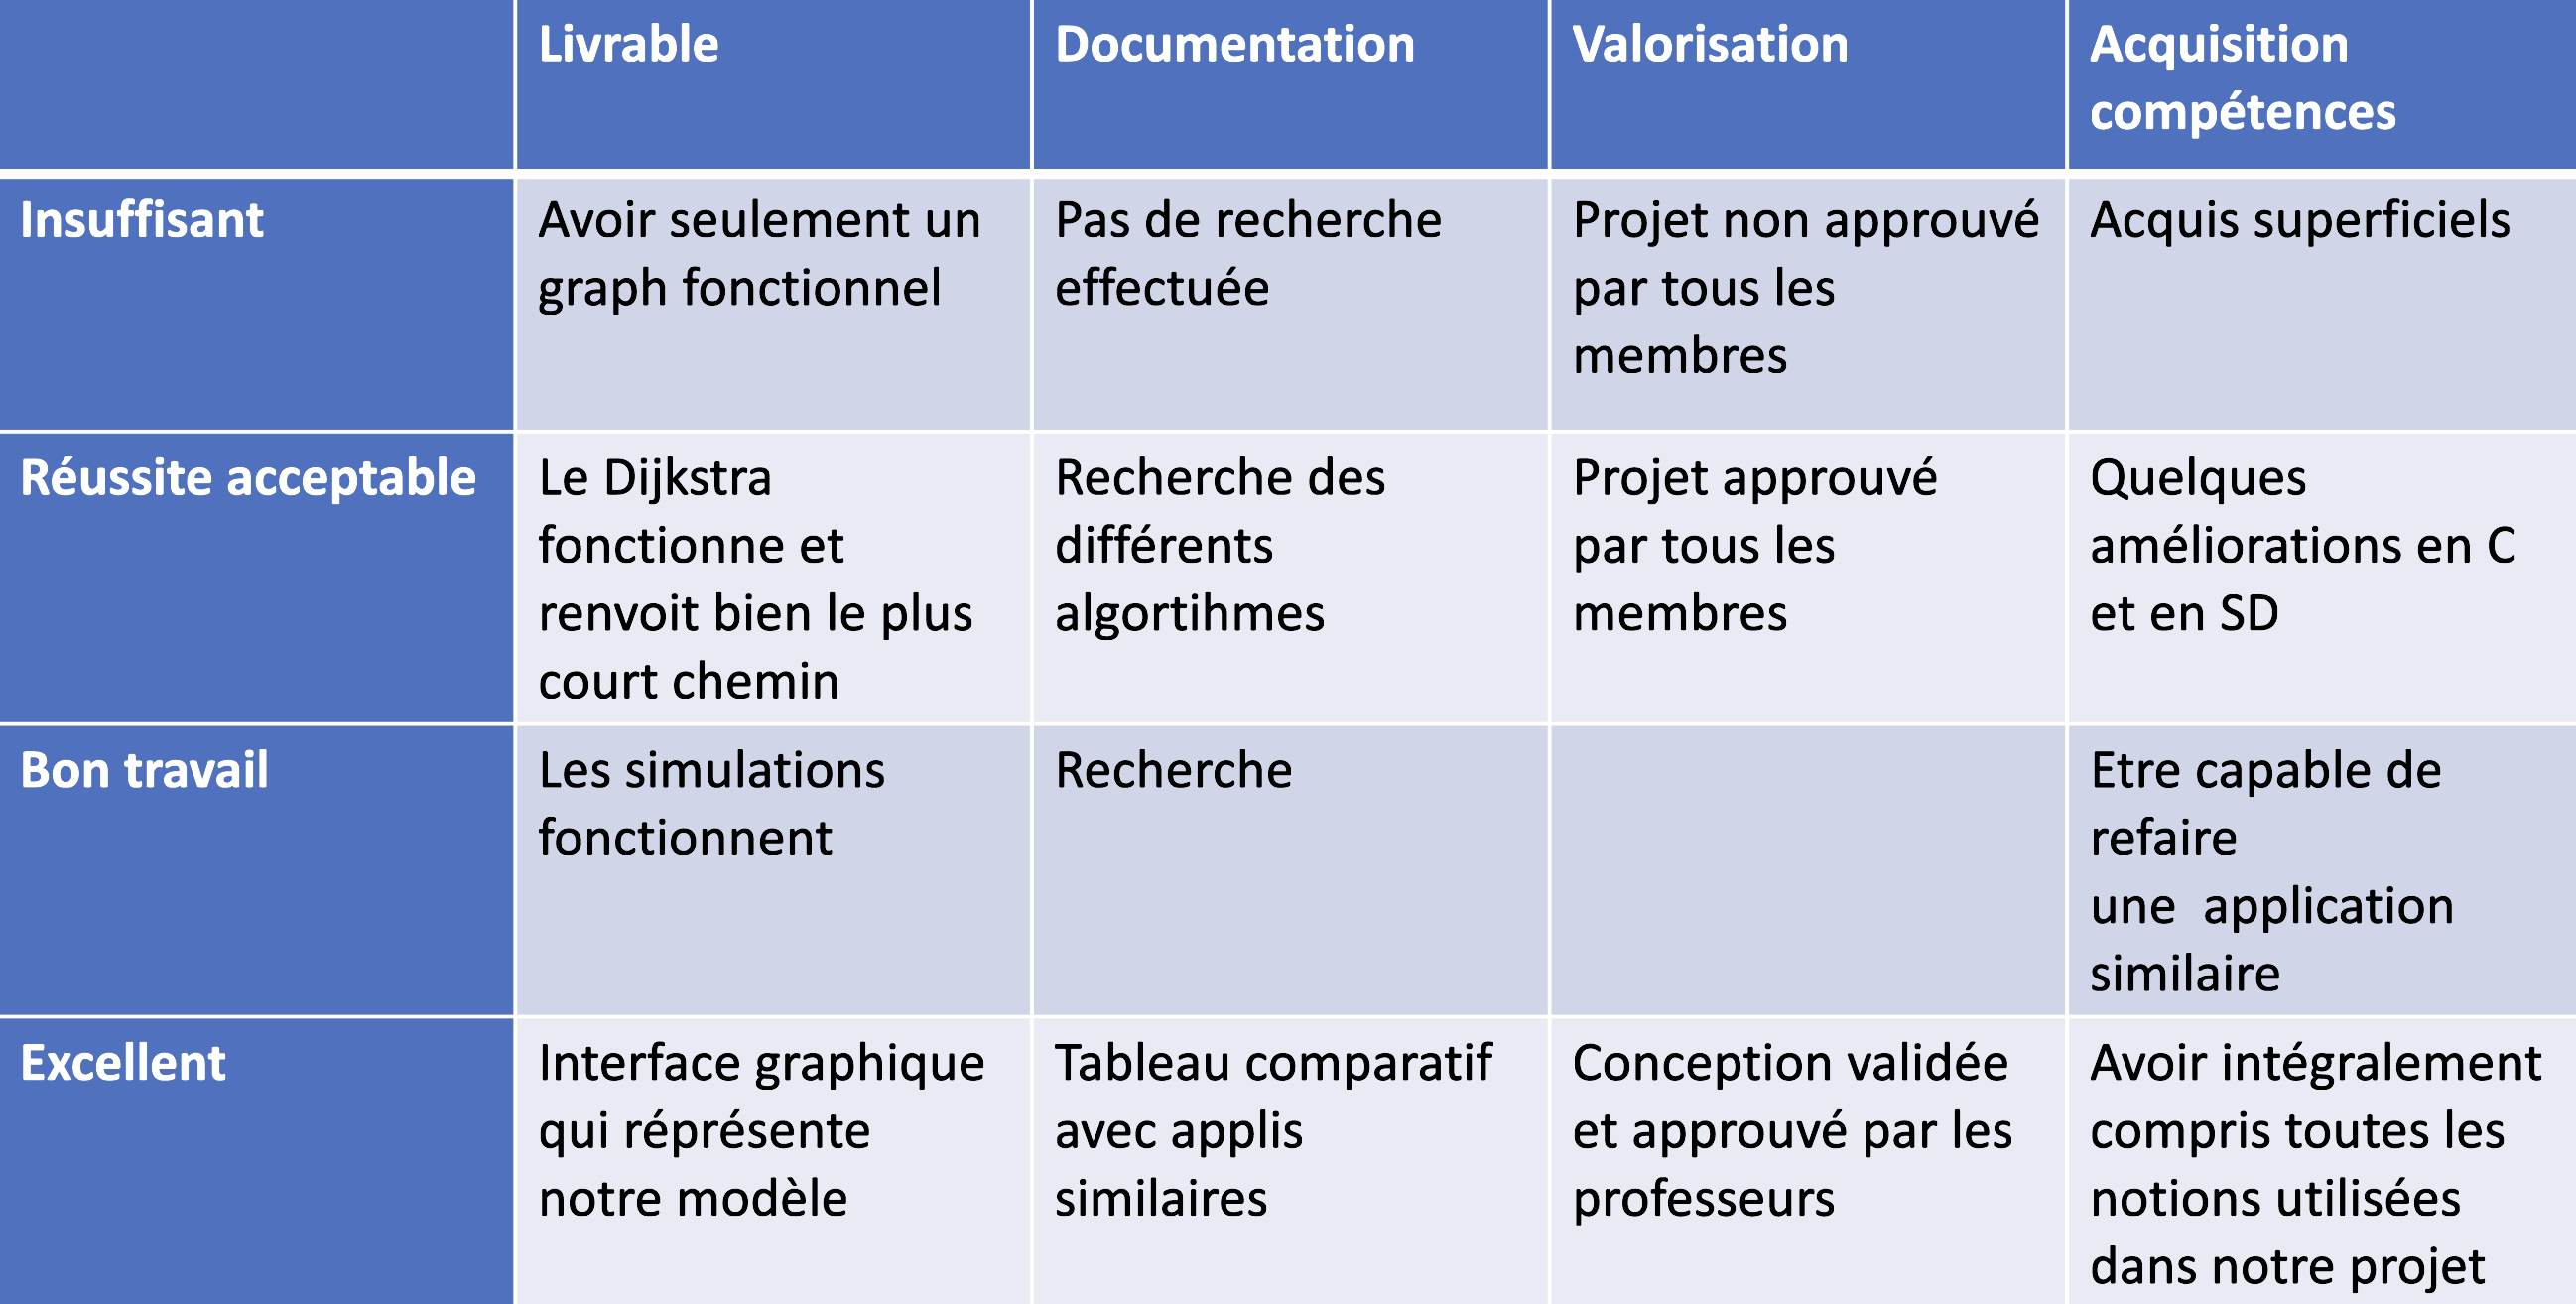
\includegraphics[width=1\textwidth]{img/matrice_des_objectifs.png}
    \caption{Matrice des objectifs}
\end{figure}

\subsection{Triangle qualité-cout-délai}
Afin d’établir des objectifs cohérents, et réalisables dans les délais, nous avons réalisé le triangle qualité-coût-délai. On remarque ainsi, les délais étant courts, que nous avons tout intérêt à ne pas se fixer des objectifs trop ambitieux sous peine de devoir renoncer à certaines fonctionnalités et de ne pas rendre le livrable annoncé initialement.

\begin{figure}[H]
    \centering
    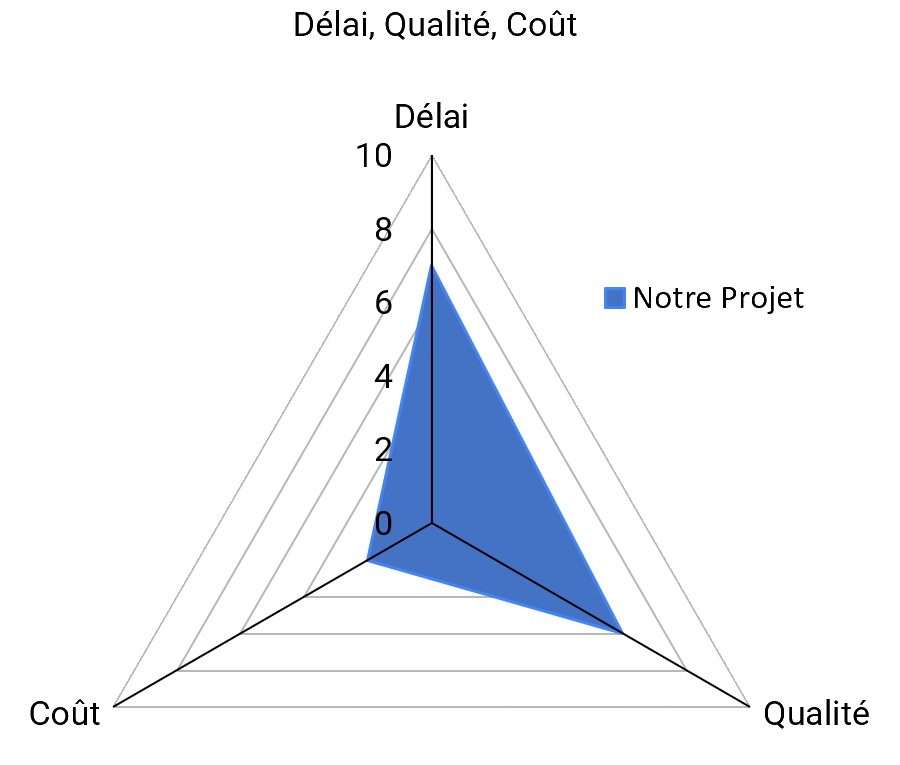
\includegraphics[width=0.5\textwidth]{img/triangle_QCD.png}
    \caption{Triangle DQC}
\end{figure}

\subsection{Matrice SWOT}
Afin d’avoir une vision plus globale de nos ressources et des facteurs internes et externes agissant sur le projet, nous avons ensuite réalisé la matrice SWOT (Strengths, Weaknesses, Opportunities, Threats) de notre projet.

\begin{figure}[H]
    \centering
    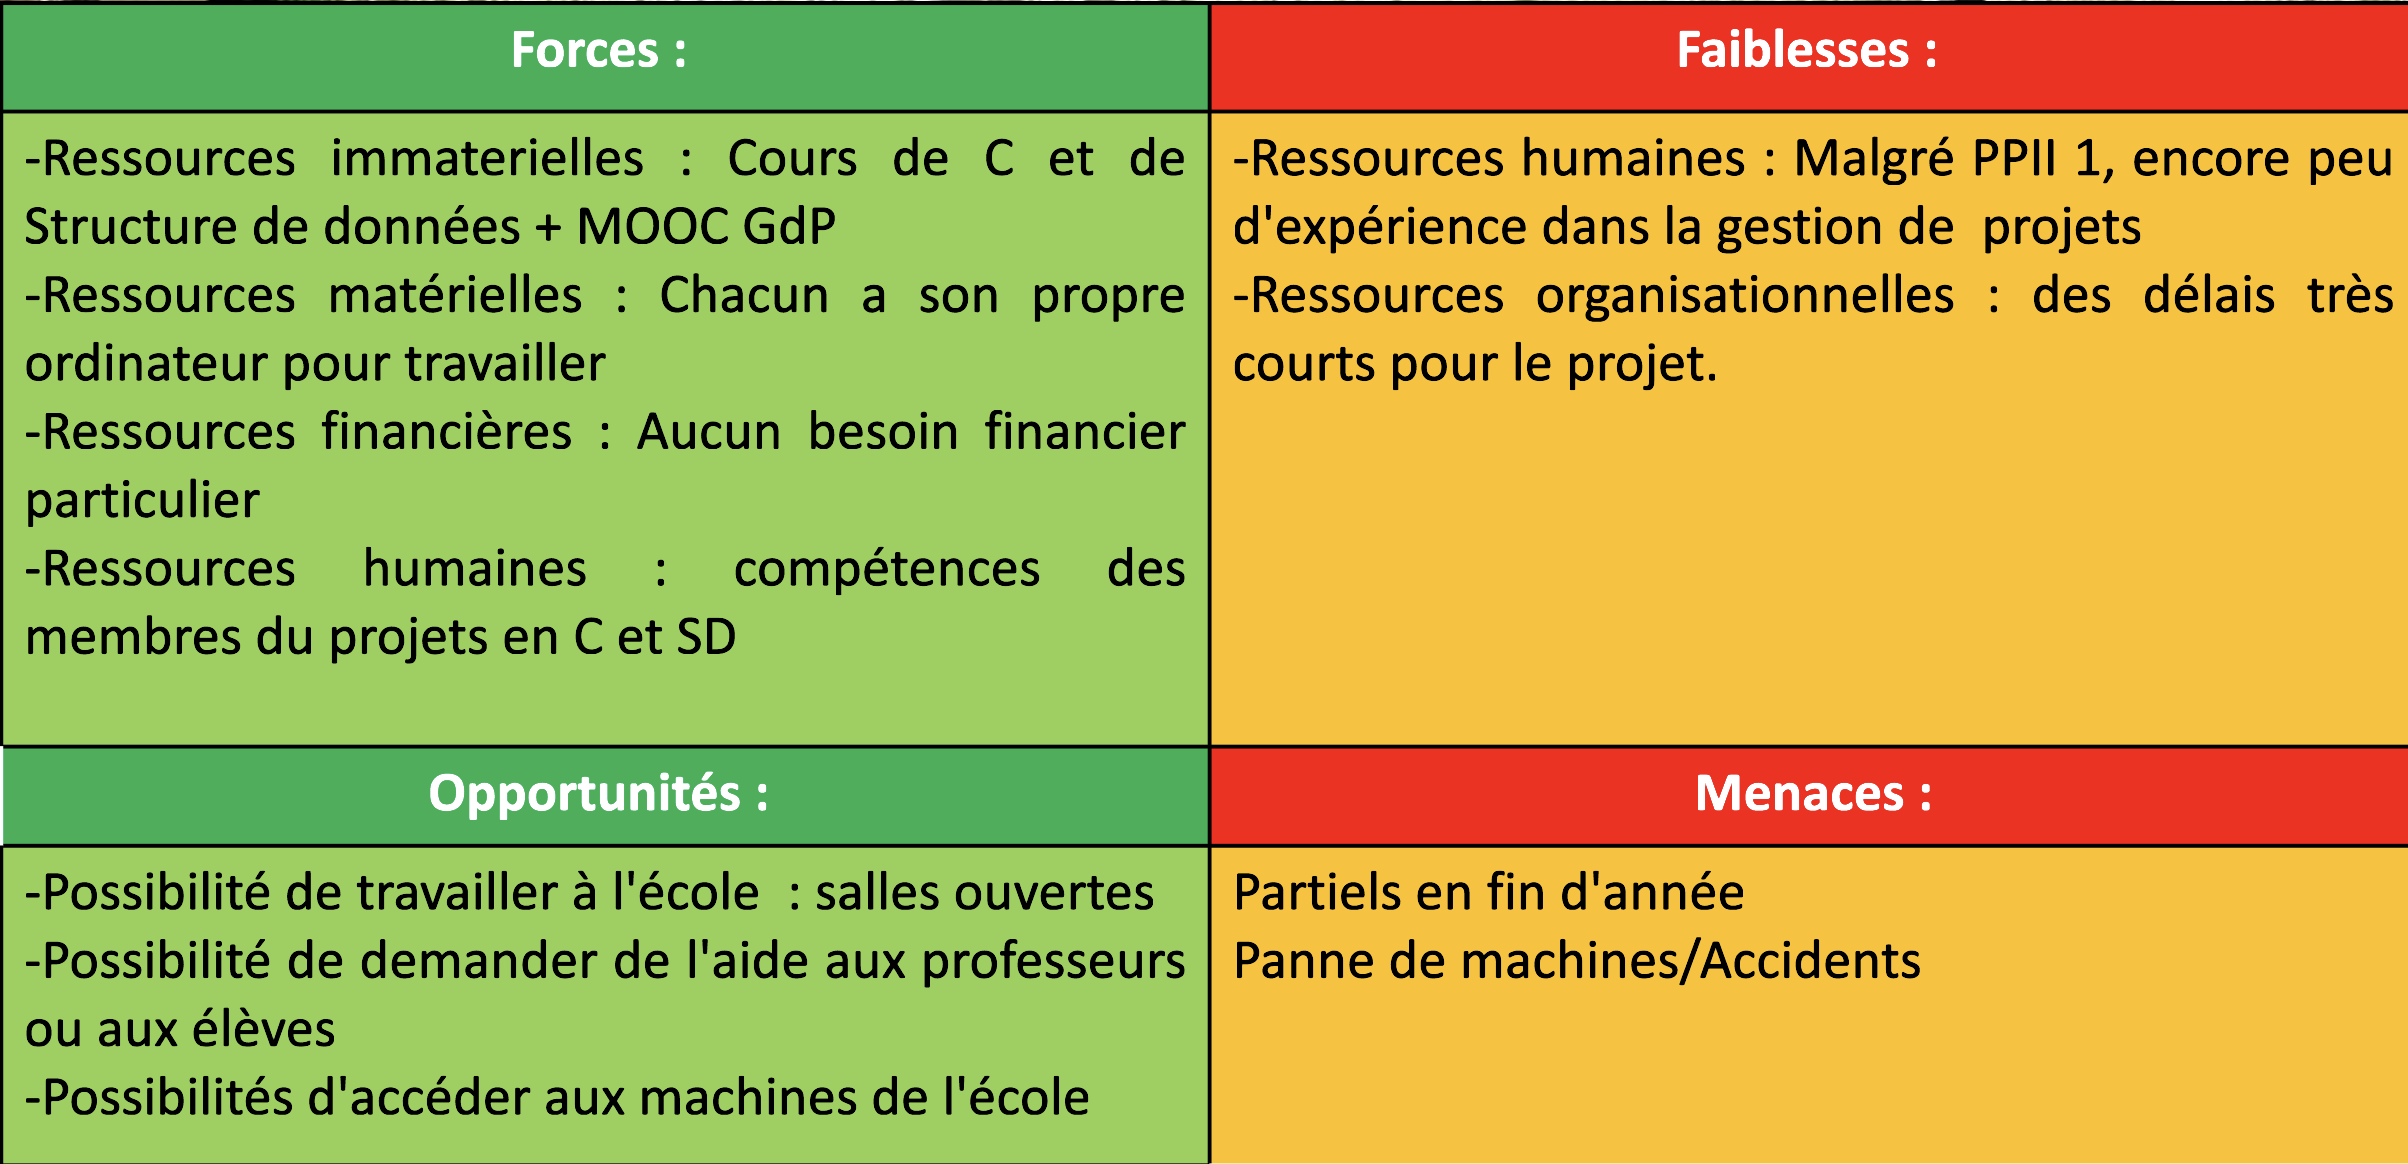
\includegraphics[width=0.75\textwidth]{img/SWOT.png}
    \caption{Matrice SWOT}
\end{figure}

On peut ainsi remarquer que notre projet présente de nombreux points forts notamment grâce aux connaissances acquises lors des cours de Télécom Nancy mais également de part l’expérience forte de deux des membres de l’équipe projet qui ont déjà réalisé des applications similaires.  Cependant, plusieurs facteurs internes constituent nos faiblesses notamment les courts délais qui nous obligent à être concis et efficaces dans notre travail, ou encore le faible bagage informatique de deux des membres de l’équipe. Néanmoins, ces lacunes constituent pour eux l’opportunité d’apprendre, et de progresser avec l’aide des membres expérimentés de l’équipe.

De plus, nous devons anticiper les charges de travail dans le cadre de notre formation à Télécom Nancy qui s'avèrent être plus élevées en décembre lors des partiels de fin d'année. Nous allons donc devoir prendre cela en compte dans notre gestion des tâches.

\subsection{Profil de projet}

Afin d’avoir une vision plus globale sur notre projet, nous avons également réalisé le profil du projet (le budget étant égal à 0, nous avons choisi de ne pas le représenter dans notre profil). On remarque que, du fait des nombreuses fonctionnalités que nous avons l’intention d’implémenter dans notre application, que notre projet est de taille moyenne mais de complexité élevée.

Cependant, les enjeux du projet ne sont pas très importants (en dehors de la note finale qui compte dans notre moyenne) car l'échec du projet n'engendrera pas la chute d'une organisation et le budget est négligeable.

De plus, au vu de l’état de l’art établi, l’innovation du projet est importante puisque nous avons choisi de combiner différentes fonctionnalités existantes de plusieurs applications et d’en rajouter de nouvelles.

\begin{figure}[H]
    \centering
    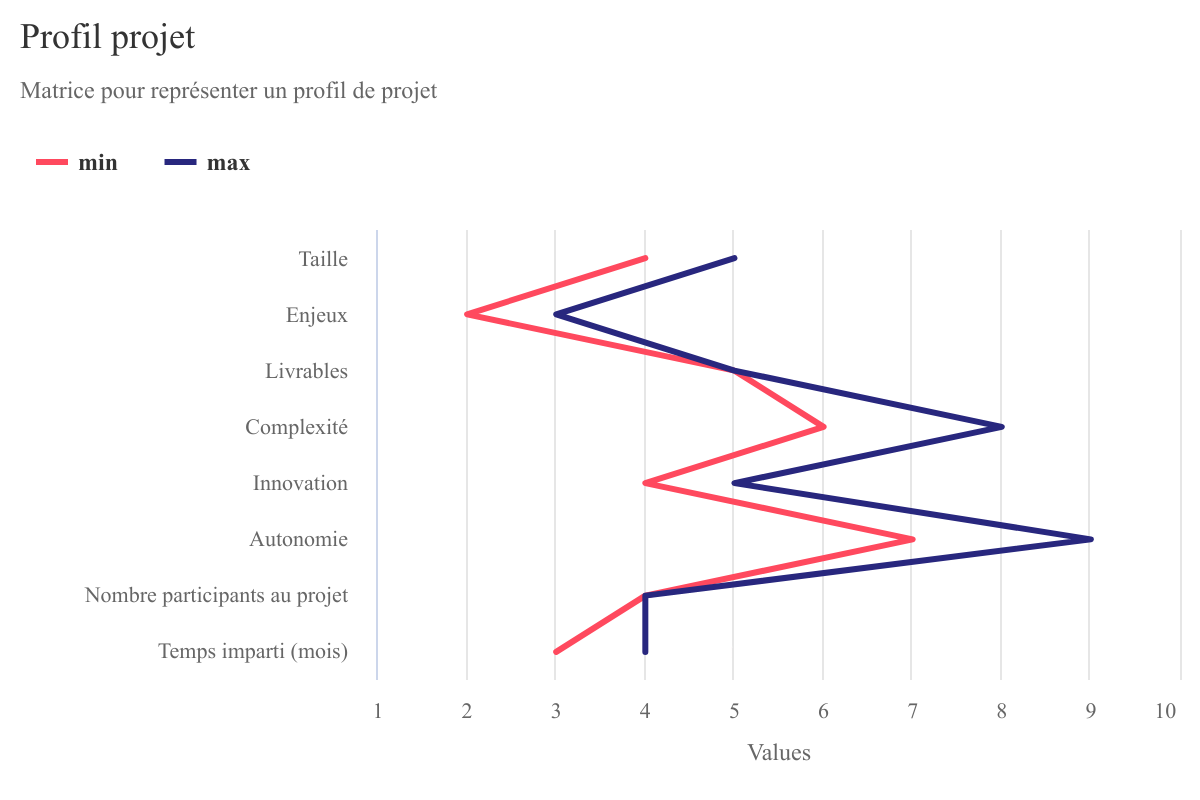
\includegraphics[width=0.75\textwidth]{img/profil_projet.png}
    \caption{Profil du projet}
\end{figure}

\subsection{WBS~: comment concrétiser l’application}
Ceci étant fait, nous avons maintenant choisi de détailler les lots de travail à effectuer pour fabriquer notre application. Nous avons ainsi réalisé le WBS (Work Breakdown Structure) de notre application~: il apparait ainsi les grandes étapes de notre projet que sont~: définition du cadre de l’application, développement des fonctionnalités de l’application et écriture du rapport.
\begin{figure}[H]
    \centering
    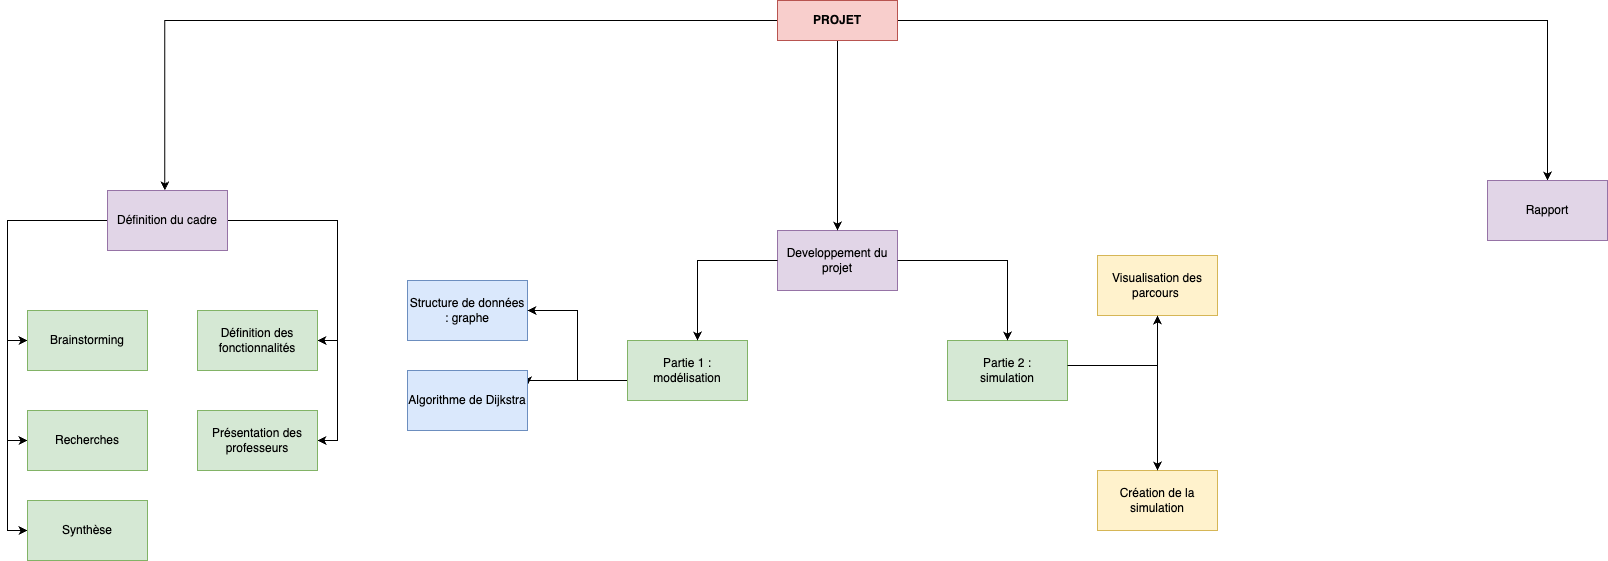
\includegraphics[width=1\textwidth]{img/WBS.png}
    \caption{WBS}
\end{figure}

\subsection{Diagramme de Gantt~: planification}
Maintenant que nous avons un détail des lots de travail qui constituent notre application, il faut maintenant les mettre en relation pour créer un planning efficace où chaque tâche est effectuée dans l’ordre.
\begin{figure}[H]
    \centering
    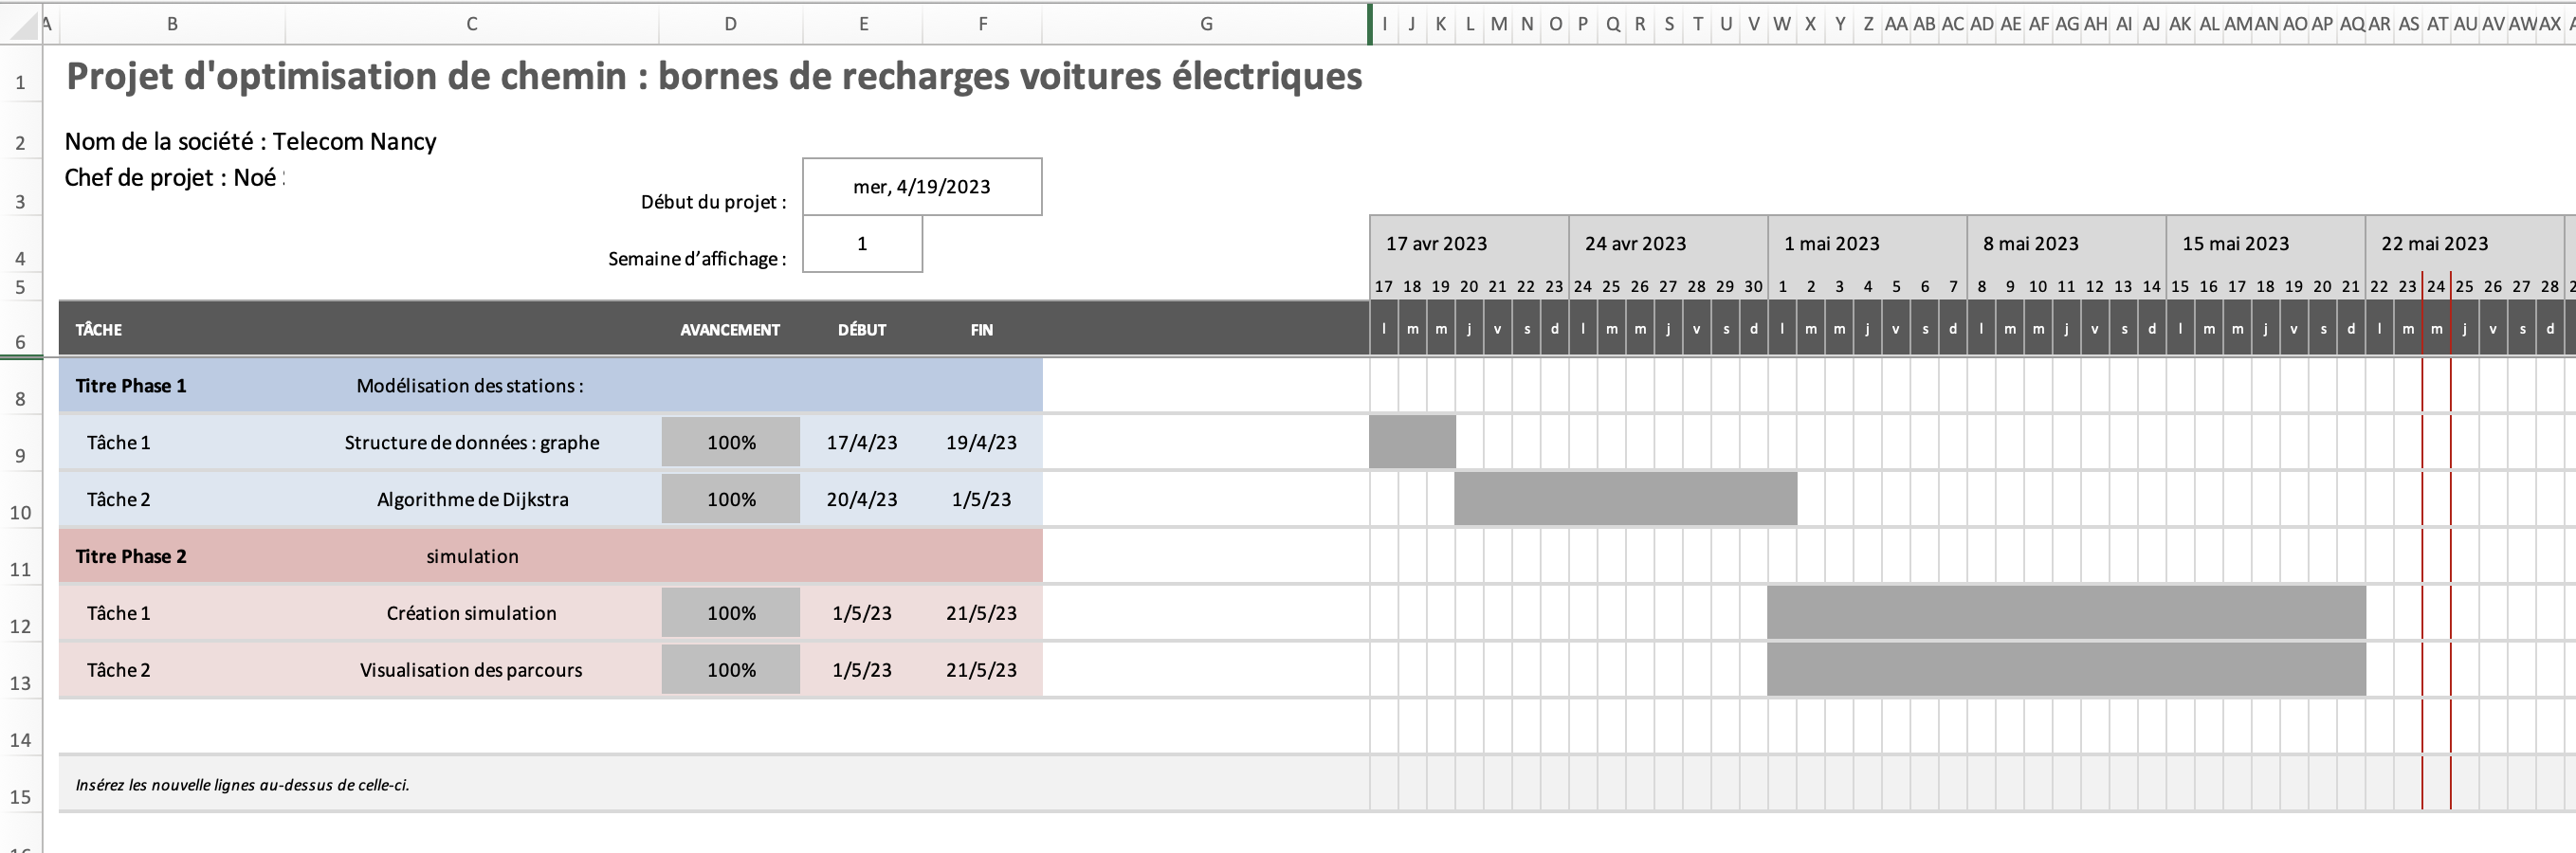
\includegraphics[width=1\textwidth]{img/gantt.png}
    \caption{Diagramme de GANTT}
\end{figure}
Ce diagramme est une première version générale des tâches à effectuer, il sera modifié et détaillé davantage une fois la conception et les maquettes du projet réalisées.

\subsection{Matrice RACI}
Maintenant que toutes les étapes sont planifiées, nous devons répartir le travail entre les membres de l’équipe. On utilise ainsi une matrice RACI synthétisant les rôles de chacun.

\begin{figure}[H]
    \centering
    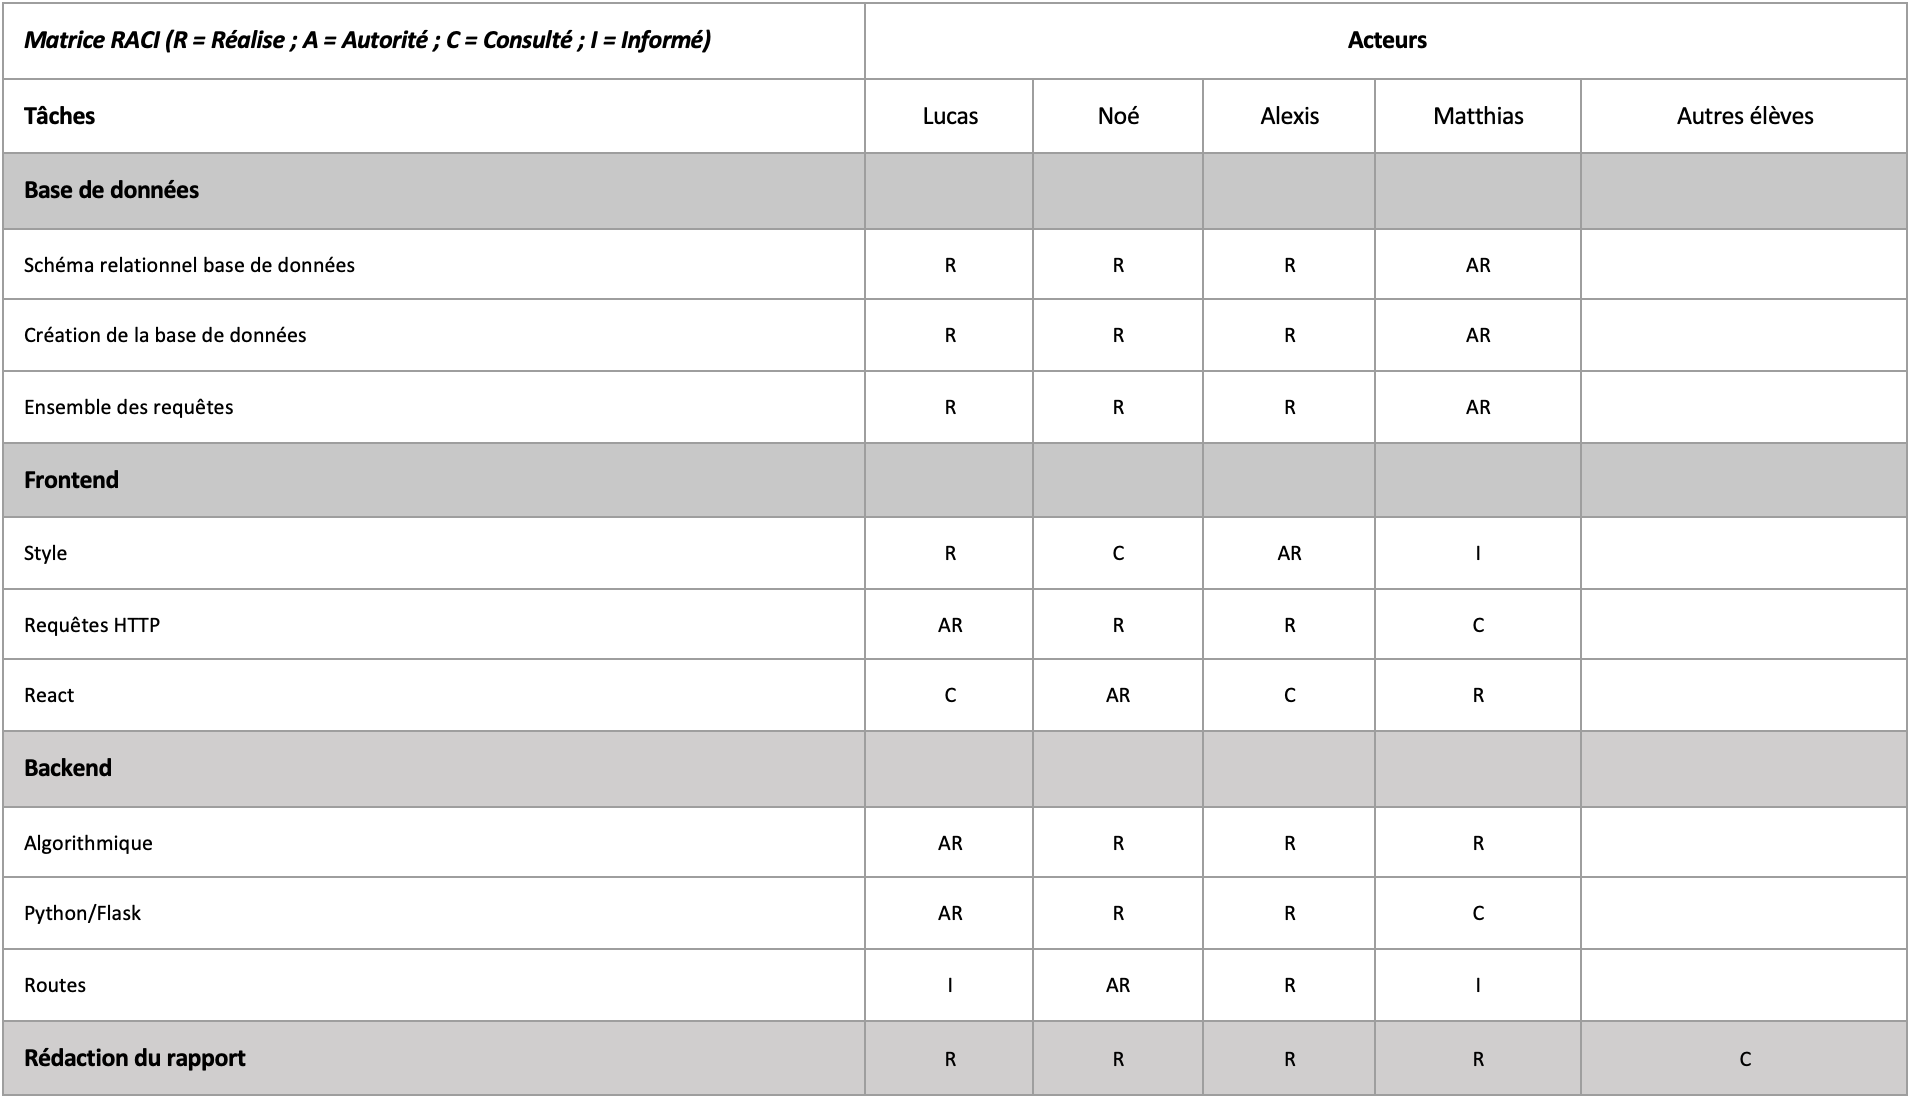
\includegraphics[width=1\textwidth]{img/RACI.png}
    \caption{Matrice RACI}
\end{figure}

\subsection{Gestion des risques}
Nous avons également pensé à prévoir une partie des risques pouvant se dresser sur notre route, les risques les plus classiques étant
la gestion du temps et le manque de compréhension de certaines personnes de l'équipe.
\begin{figure}[H]
    \centering
    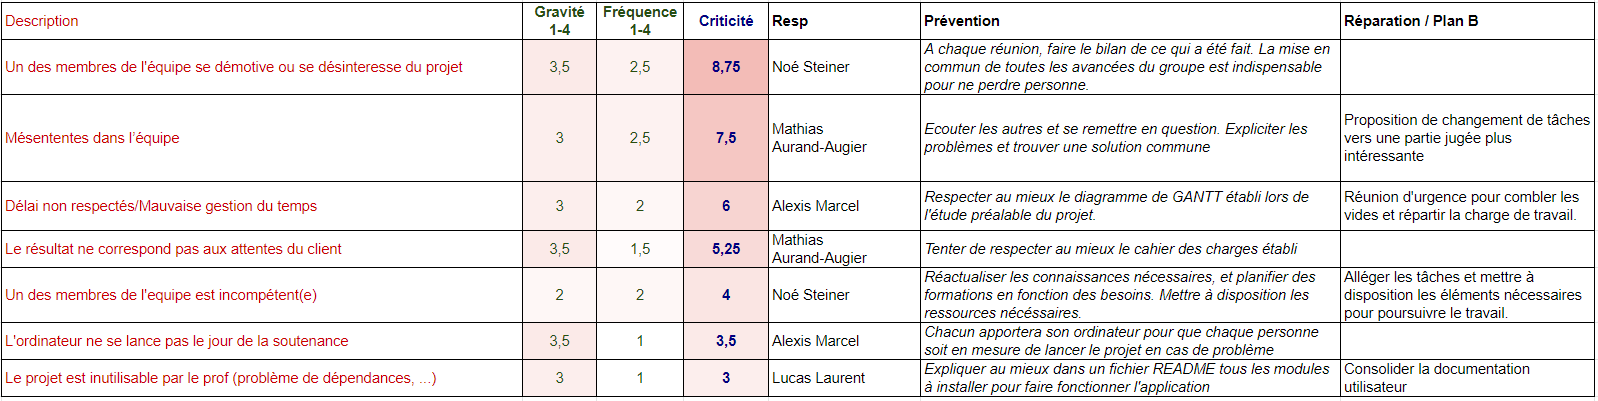
\includegraphics[width=1\textwidth]{img/Plan_gestion_risque.png}
    \caption{Plan de gestion des risques}
\end{figure}

\section{Conclusion}
Ce projet nous a permis de réaliser un projet de A à Z, de la conception à la réalisation. Nous avons pu mettre en pratique les connaissances acquises en cours et nous avons pu nous familiariser avec les outils de gestion de projet. Nous avons également pu nous rendre compte de la difficulté de la gestion de projet et de la nécessité de bien planifier son travail.
Nous avons réalisé la totalité des fonctionnalités et des éléments prévus lors de la phase de conception, ce qui nous permet de qualifier notre travail d'excellent selon notre matrice des objectifs.
Ce travail a également été l'occasion de découvrir de nouvelles technologies, comme les librairies React, Gurobipy et SQLAlchemy, mais également de découvrir de nouvelles méthodes de résolution de problème, via notre algorithme d'optimisation de l'arrosage.
Nous sommes fiers du rendu final de notre travail et espérons retravailler ensemble sur d'autres projets, y compris externes à ceux donnés dans le cadre des cours.
\section{Annexes}
\includepdf[pages=1]{../../cr_reu/octobre/16/cr_16_octobre.pdf}
\includepdf[pages=1]{../../cr_reu/octobre/18/cr_18_octobre.pdf}
\includepdf[pages=1]{../../cr_reu/novembre/18/cr_18_novembre.pdf}
\includepdf[pages=1]{../../cr_reu/novembre/30/cr_30_novembre.pdf}
\includepdf[pages=1]{../../cr_reu/decembre/16/cr_16_decembre.pdf}
\includepdf[pages=1]{../../cr_reu/decembre/20/cr_20_decembre.pdf}
\includepdf[pages=1]{../../cr_reu/decembre/23/cr_23_decembre.pdf}
\includepdf[pages=1]{../../cr_reu/decembre/27/cr_27_decembre.pdf}
\end{document}